% It is an example file showing how to use the 'acm_proc_article-sp.cls' V3.2SP
% LaTeX2e document class file for Conference Proceedings submissions.
\documentclass{edm_template}

% Somehow the desired top margin is being set to 1/16in?
\addtolength{\topmargin}{0.6875in}

\usepackage{graphics}

\begin{document}

\title{Applying three models of learning to individual student log data}
\numberofauthors{1}
\author{
\alignauthor
      Brett van de Sande\\
       \affaddr{Arizona State University}\\
       \affaddr{PO Box 878809}\\
       \affaddr{Tempe, AZ~~85287}\\
       \email{bvds@asu.edu}
}

\maketitle

\begin{abstract}
Normally, when considering a model of learning, one compares the model
to some measure of learning that has been aggregated over students.
What happens if one is interested in individual differences?  For
instance, different students may have received different help, or may
have behaved differently.  In that case, one is interested in
comparing the model to the individual learner.  In this study, we
investigate three models of learning and compare them to student log
data with the goal of seeing which model best describes individual
student learning of a particular skill.  The log data is from students
who used the Andes intelligent tutor system for an entire semester of
introductory physics.  We discover that, in this context, the "best
fitting model" is not necessarily the "correct model" in the usual
sense.
\end{abstract}

\keywords{data mining, models of student learning}


\section{Introduction}

%Talk about ultimate goal of using this to determine effectiveness
%of help given or of a particular student behavior.

Most Knowledge Component (KC) \cite{vanlehn_behavior_2006}
based models of learning are constructed
in a similar manner, following Corbett and Anderson~\citeyear{corbett_knowledge_1995}.
First, some measure of learning is selected ({\em e.g.} correct/incorrect
on first try) for the $j$-th opportunity for that student to apply a given KC.  
This measure of learning is then aggregated over students 
({\em e.g.} fraction of students correct) as a function of $j$.
Finally, aggregated measure is then compared to some model
({\em e.g.} Bayesian Knowledge Tracing) with model parameters
chosen to optimize the model's fit to the data.
In principle, given sufficient student log data, one could uniquely
determine which of several competing models best matches the
data.

One drawback with this approach is that it does not take into account
individual learner differences or the actual behaviors of students or
tutors as they are learning.  Thus, a number of authors have extended
their models to include individual student proficiency and actual help
received by the student.  For instance, in the Cordillera natural
language tutoring system for physics~\cite{vanlehn_developing_2007},
the student may have been asked what the next step was or were told
what the next stop was; this was used as input for an associated
model.  An overview of these models can be found 
in~\cite{chi_instructional_2011}.

If one is primarily interested in the effectiveness of help given to
an individual student or the effectiveness (for learning) of a particular
strategy or behavior of a the student, then it may make sense
to fit a model of learning to the log data of each student individually.
Given sufficient student log data, can we still talk about a particular
model fitting the student log data well?  That is the central question
of this paper.
To start our investigation, we will compare three different models of
learning using data from students taking introductory physics and examine
whether there is empirical support for using one model over the
others.  In fact, using Akaike Information Criteria (AIC), we obtain
results that seem to favor two models over the third, but note
that fitting the models to individual students can make the determination ambiguous.


\subsection{Correct/Incorrect steps}

Our stated goal is to determine student learning for an individual
student as they progress through a course.  What observable quantities
should be used to determine student mastery?  One possible observable
is ``correct/incorrect steps,'' whether the student correctly applies
a given skill at a particular problem-solving step without any
preceding errors or hints.  There are other observables that may give
us clues on mastery: for instance, how much time a student takes to
complete a step that involves a given skill.  However, other such
observables typically need some additional theoretical
interpretation. {\em Exempli gratia}, What is the relation between
time taken and mastery?  Baker, Goldstein, and
Heffernan~\citeyear{baker_detecting_2011} develop a model of learning
based on a Hidden Markov model approach.  They start with a set of
% BvdS:  use actual number.
25 additional observables (including ``time to complete a step'') and
construct their model and use correct/incorrect steps
to calibrate the additional observables and determine which are
significant.  Naturally, it is
desirable to eventually include various other observables in any
determination of student learning.  However, in the present investigation,
we will focus on correct/incorrect steps.

Next,  we need to define
precisely what we mean by a step.
A student attempts some number of {\em steps} when solving a problem
using an intelligent tutor system (ITS).
Usually, a step is associated with creating/modifying a single user
interface object (writing an equation, drawing a vector, defining a
quantity, {\em et cetera}) and is a distinct part of the problem
solution (that is, help-giving dialogs are not considered to be
steps).  A student may attempt a particular problem-solving step,
delete the object, and later attempt that solution step again.  A step
is an {\em opportunity} to learn a given Knowledge Component
(KC)~\cite{vanlehn_behavior_2006} if the student must apply that skill
to complete the step.

%
%  Not needed in this paper.
%
%Each step $j$ corresponds some some number of student-tutor 
%{\em transactions}: attempts at constructing the associated object, 
%or associated interactions with the Andes help system.  

%Next, we need a model of student learning for a particular KC.
%Since the policies chosen by the random-help version of Andes
%are different for each student,
%we need to determine the point of learning for each student.
For each KC and student, we select all attempted steps that involve application
of that KC and mark each step as ``correct'' if
the student completes that step correctly without any preceding errors or 
requests for help; otherwise, we mark the step as ``incorrect.''
\label{steps}  % Section reference for correct/incorrect
If each incorrect/correct step is marked with a 0/1, then
a single student's performance on a single KC can be expressed as a bit  sequence,
{\em exempli gratia} 00101011.  We will label
steps with $j\in\left\{1,\ldots,n\right\}$.  

\section{Three models of learning}

\begin{figure}
  \centering 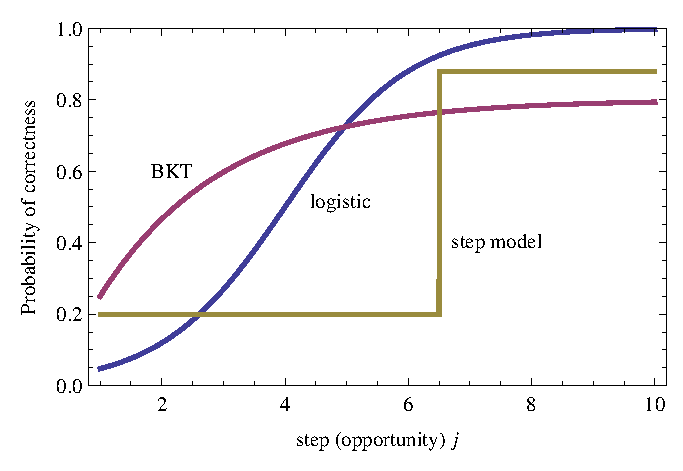
\includegraphics{three-models.eps}
  \caption{Functional form of the three models of student learning.}
    \label{three-models}
\end{figure}

Ultimately, we are interested in determining when a student has mastered
a particular KC and, by inference, the effectiveness of
any help given by the tutor.  Thus, a useful model of learning
should  have the the following properties:
\label{model-criteria}
%
\begin{enumerate} 

\item Be compatible with actual student behavior.
      That is, its
      functional form should fit well with student data.
      We will explore this question in Section~\ref{model-selection}.  

\item \label{crit:step}
      Give the probability that learning has occurred at a given step.

\item  \label{crit:perform}
     Assuming learning has occurred at a given step, the model
     should give a prediction for the 
     associated increase in performance and 
     the rate of errors after learning.

\end{enumerate}
%
We will consider three candidate models:  
the Bayesian Knowledge Tracing (BKT) model, the logistic function,
and the ``step model;''
see Fig.~\ref{three-models}.



The first model is the Bayesian Knowledge Tracing (BKT) 
model~\cite{corbett_knowledge_1995}.  The hidden Markov model
form of BKT is often fit to student performance 
data~\cite{beck_identifiability:_2007}.  One can show that
this model, in functional form, is an exponential function
with three model parameters~\cite{van_de_sande_properties_2012}:
%
%  A and \beta are kind of messy, so we don't include them here.
\begin{equation}
         P_\mathrm{BKT}(j) = 1-P(S) -A e^{-\beta j} \; .
\end{equation}
%
One central assumption of BKT is that, given that learning
has not already occurred, mastery is {\em equally probable} on each step.
This assumption of equal probability does not match well with 
our goal of determining empirically the steps where learning has 
actually occurred for an individual student, criterion~\ref{crit:step}.
On the other hand, this model does provide the final
error rate $P(S)$ (the initial error rate is ambiguous), 
so criterion~\ref{crit:perform} is partially satisfied. 

Another model that is frequently used in the context of learning is
the logistic model~\cite{cen_learning_2006,chi_instructional_2011},
%
\begin{equation}
    P_\mathrm{logistic}(j)= \frac{1}{1+\exp\left(-b (j-L)\right)} \; .
\end{equation}
%
It is natural to associate $L$ with the moment of learning.  However,
the finite slope of $P_\mathrm{logistic}(j)$ means that learning may
occur in a range of roughly $1/b$ steps before and after $L$.  For
$P_\mathrm{logistic}(j)$, the gain in performance is always 1 and the
final error rate is always 0.  Thus, although this model makes a
prediction for when the skill is learned, criterion~\ref{crit:step},
it does not predict a gain in performance,
criterion~\ref{crit:perform}.

The third model is the ``step model'' which assumes that learning 
occurs all at once; this corresponds to the ``eureka learning''
discussed by \cite{baker_detecting_2011}.  It is defined as:
%
\begin{equation}
    P_\mathrm{step}(j)= \left\{\begin{array}{cc}
                 g, & j<l \\
                 1-s, & j\ge L 
                 \end{array} \right. 
\end{equation}
%
where $L$ is the step where the student first shows mastery of the KC,
$g$ is the ``guess rate,'' the probability that the student gets a
step correct by accident, and $s$ is the ``slip rate,'' the chance
that the student makes an error after learning the skill.  These are
analogous to the guess and slip parameters of
BKT~\cite{corbett_knowledge_1995}.  The associated gain in performance
is $1-g-s$ and the error rate after learning is simply $s$ in this
model.  Thus, this model satisfies criteria \ref{crit:step} and
\ref{crit:perform}.

\section{Model selection using AIC}
\label{model-selection}

The BKT and logistic function models are widely used and
we have introduced the step model $P_\mathrm{step}(j)$
as an alternative.  How
well do these models match actual student behavior?
Since we will use the step model in subsequent
work, it would be reassuring to know whether it describes the student data as 
well (or better than) the other two models.  We will use the Akaike Information Criterion (AIC) for this purpose~\cite{akaike_new_1974,burnham_model_2002}.
AIC is defined as
%
\begin{equation}
   \mathrm{AIC}= -2 \log\left(\mathcal{L}\right) + 2K
\end{equation}
% 
where $\mathcal{L}$ is the maximized value of the likelihood function
and $K$ is the number of parameters in the model.
 AIC is an estimate of the expected relative ``distance''
between a given model and the true model (assumed to be complicated) 
that actually generated the observed data.  It is valid in limit of 
many data points, $n\to\infty$, with leading corrections of order $1/n$.

A related method for choosing between models is the Bayesian
Information Criterion (BIC) introduced by
Schwarz~\citeyear{schwarz_estimating_1978}.  BIC is defined as
%
\begin{equation}
   \mathrm{AIC}= -2 \log\left(\mathcal{L}\right) + K \log\left(n\right)
\end{equation}
% 
where $n$ is the number of data points.
Burnham \& Anderson~\citeyear[Sections~6.3 \& 6.4]{burnham_model_2002} explain
that BIC is more appropriate in cases where the ``true'' model that
actually created the data is relatively simple (few parameters).  If
the true model is contained in the set of models being considered,
then BIC will correctly identify the true model in the $n\to\infty$
limit.  For BIC to have this property, the true model must stay fixed as 
$n$ increases.  
The authors argue that, while BIC may be appropriate in some
of the physical sciences and engineering, in the biological and social
sciences, medicine, and other ``noisy'' sciences, the assumptions that
underlie BIC are generally not met.  In particular, as the sample size
increases, it is typical that the underlying ``true'' model also
becomes more complicated.  This is certainly true in educational
datamining: datasets are generally increased by adding data from new schools, or
different years and one generally expects noticeable variation of student
behavior from school to school or from year to year.  In such cases, one
safely can say that the ``true'' model is complicated (because people are
complicated) and becomes more complicated as a dataset is increased in
size.  Although most authors quote both AIC and BIC values, there
is good reason to believe that AIC is generally more appropriate for
educational datamining work.

\subsection{Method}

\begin{figure}
  \centering 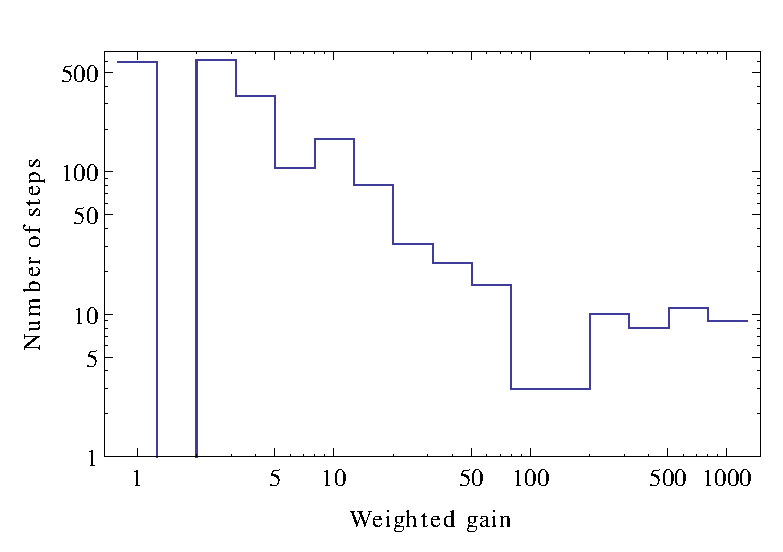
\includegraphics{student-kc-length-histogram.eps}
  \caption{Histogram of number of distinct student-KC sequences in student 
    dataset $\mathcal{A}$ having a given number of steps $n$.}
    \label{student-length-histogram}
\end{figure}

We examined log data from 12 students taking an intensive introductory
physics course at St.\ Anselm College during summer 2011.  The course
covered the same content as a normal two-semester introductory course.
Log data was recorded as students solved homework problems while using
the Andes intelligent tutor homework system.  231 hours of log data
were recorded.
%, covering 85,744 transactions, and 26,204 student steps.  
Each step was assigned to one or more different KC's.  The dataset
contains a total of 2017 distinct student-KC sequences covering a total of
245 distinct KC's.  We will refer to this dataset as student dataset
$\mathcal{A}$.  See Figure~\ref{student-length-histogram} for a
histogram of the number of student-KC sequences having a given number of
steps.

Most KC's are associated with physics
or relevant math skills while others are associated with 
Andes conventions or user-interface actions (such as, notation
for defining a variable).  The student-KC sequences with the largest 
number of steps are associated with user-interface related skills,
since these skills are exercised throughout the entire course. 

One of the most remarkable properties of the distribution in
Fig.~\ref{student-length-histogram} is the large number of
student-KC sequences containing just a few steps.
The presence of many student-KC sequences with just one or two
steps may indicate that the default cognitive model associated 
with this tutor system may be sub-optimal; to date, there has not 
been any attempt to improve on the cognitive model of 
Andes with, say, Learning Factors Analysis~\cite{cen_learning_2006}.
Another contributing factor is the way that introductory physics is 
taught in most institutions, with relatively little repetition of 
similar problems.  This is quite different than, for instance, 
a typical middle school math curriculum where there are a large number
of similar problems in a homework assignment.

\subsection{Analysis}

\begin{figure}
  \centering 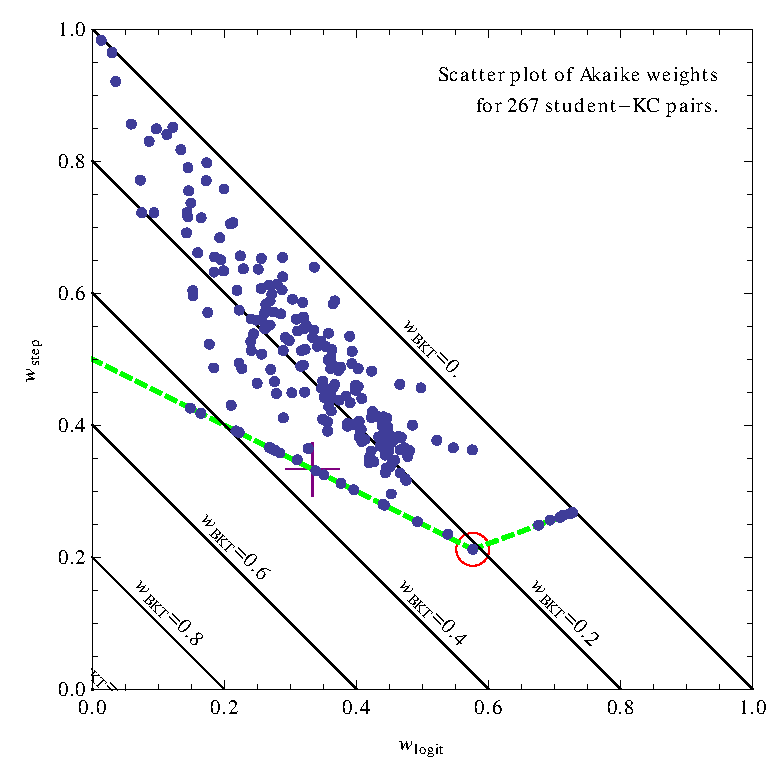
\includegraphics{scatter-weights.eps}
  \caption{Scatter plot of  Akaike weights for the three models, 
   $P_\mathrm{step}$, $P_\mathrm{logistic}$, and $P_\mathrm{BKT}$, 
   when fit to student-KC sequences from an introductory physics course.
   The point where all models are equal,
   $w_\mathrm{step}=w_\mathrm{logistic}=w_\mathrm{BKT}=1/3$, is
   marked with the lower cross.  
   The average of the  weights is marked with
   the upper cross.
  The dashed line on the left represents points
   where $w_\mathrm{step}=w_\mathrm{BKT}$.  Finally, the dashed line on 
   the right marks data with bit sequences of the form
   $00\cdots 011\cdots 1$.} 
   \label{scatter1}
\end{figure}

% LaTeX is very sensitive to the placement of this figure
\begin{figure*}
  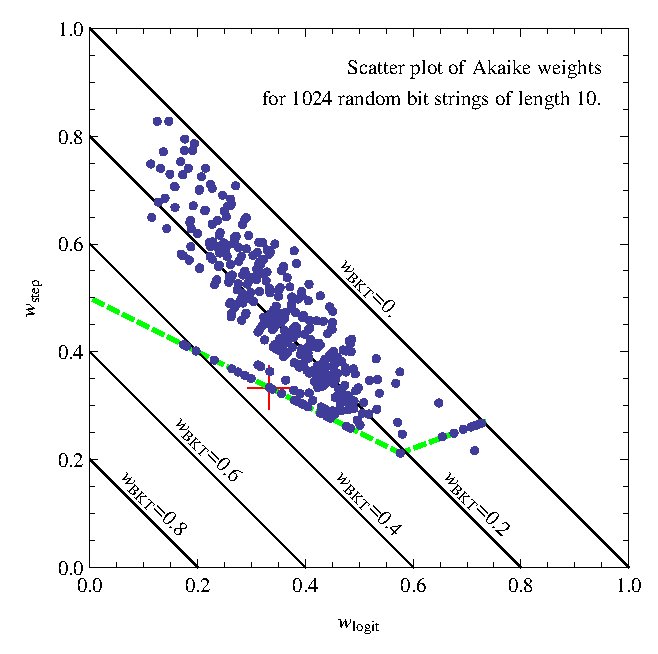
\includegraphics{scatter10.eps}
  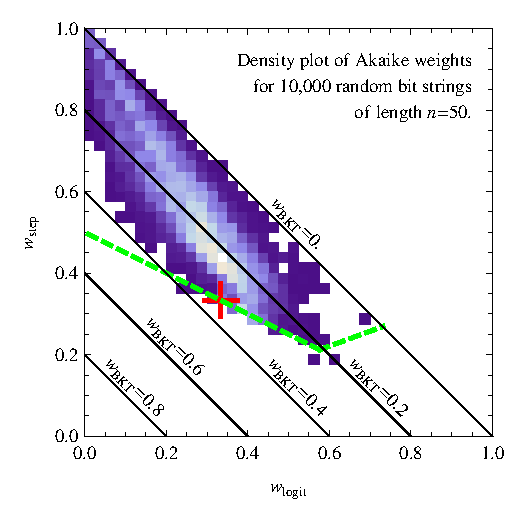
\includegraphics{density50.eps}
  \caption{Akaike weights for the three models, 
   $P_\mathrm{step}$, $P_\mathrm{logistic}$, and $P_\mathrm{BKT}$, 
   when fit to randomly generated data.  The point where
   $w_\mathrm{step}=w_\mathrm{logistic}=w_\mathrm{BKT}=1/3$ is
   marked with a cross.  For these datasets, each 
   model should perform equally well, since, with an appropriate
   choice of parameters, they all can be made equal to 
   the model that was used to generate the data.}\label{scatter2}
\end{figure*}

Since the goodness of fit criterion, AIC, is valid in the limit of
many steps, we include in this analysis only student-KC sequences that
contain 10 or more steps, reducing the number of student-KC sequences
to 267, covering 38 distinct KC's.  We determine the correctness of
each step (Section~\ref{steps}), constructing a bit sequence, {\em
exempli gratia} 001001101, for each student-KC sequence.  This bit
sequence is then fit to each of the three models, $P_\mathrm{step}$,
$P_\mathrm{logistic}$, and $P_\mathrm{BKT}$ by maximizing the
associated log likelihood.  %This determines the free parameters in
each model.  We then calculate the AIC score for each fit.  Finally,
we calculate the Akaike weights, $w_\mathrm{logistic}$,
$w_\mathrm{step}$, and $w_\mathrm{BKT}$ for each student-KC
sequence~\cite{burnham_model_2002}.
The weights are normalized so that
%
\begin{equation}
   1=w_\mathrm{logistic}+ w_\mathrm{step} + w_\mathrm{BKT} \; .
\end{equation}
%
The Akaike weight represents the relative probability that
a particular model in a given set of models is closest
to the model that has actually generated the data. 

A scatter plot of the weights is shown in Fig.~\ref{scatter1}.
If all three models described the data equally well, then
we would expect points to be scattered evenly about 
center point $w_\mathrm{logistic}= w_\mathrm{step}= w_\mathrm{BKT}=1/3$.
Instead, we see the step model (average weight 0.44) weakly 
favored over the logistic model (average weight 0.37) and 
strongly favored over BKT (average weight 0.18).  Indeed, we 
find no data points where $w_\mathrm{step}< w_\mathrm{BKT}$,
although there is a noticeable accumulation of points along the line 
$w_\mathrm{step}= w_\mathrm{BKT}$.

Note that data in the form of incorrect steps then correct steps, 
{\it exempli gratia} $00\cdots 011\cdots 1$,
is fit perfectly by both the $P_\mathrm{step}$ and 
$P_\mathrm{logistic}$ models.  
In this case, since $P_\mathrm{logistic}$ has one fewer parameter
than $P_\mathrm{step}$, it is favored by AIC by a constant factor and
$w_\mathrm{step}=\mathrm{e}^{-1} w_\mathrm{logistic}$.  This case is
plotted as the increasing dashed line in Fig.~\ref{scatter1}.

Since the student-KC sequences contain an average of about $n=16$ 
steps, it is surprising that we find that AIC so strongly
discriminates between the models.  Perhaps, though,  this is due to
some finite $n$ correction:  recall that AIC is only 
strictly valid in the $n\to\infty$ limit.

\subsection{Random data}


To further investigate the observed strong discrimination
between the three models, we constructed an
artificial dataset containing random bit sequences (each
step has 50\% probability of being ``correct'') of length 
$n\in\left\{10,20,30,40,50\right\}$.
This dataset corresponds to a model of the form
%
\begin{equation}
        P_\mathrm{random}(j)=1/2 \; .
\end{equation}
%
We then repeated our analysis of the three models using this dataset
and AIC as our selection criterion.  Note that all three models,
with a suitable choice of parameters, can be made equal to 
$P_\mathrm{random}$ itself.


As mentioned earlier, for data that is generated by a simple 
model (and $P_\mathrm{random}$ is about as
simple as one can get) and the ``true'' model is included among
the set of models, BIC is the more appropriate criterion
for model selection~\cite[Sections~6.3 \& 6.4]{burnham_model_2002}.
However, for our results, the only difference between AIC and BIC 
is that BIC favors $P_\mathrm{logistic}$ more strongly over 
$P_\mathrm{step}$ and $P_\mathrm{BKT}$.  Thus, using BIC would shift 
the weights so that $w_\mathrm{logistic}$ would increase somewhat over 
the other two weights.  However, in order to maintain consistency with
our experimental results, Fig.~\ref{scatter1}, we used AIC for the random data as well;
see Fig.~\ref{scatter2}.  This use of AIC versus BIC does not 
affect our conclusions.

For data generated by $P_\mathrm{random}$,
one expects that all three models should perform equally
well since all three can equal (with suitable choice of parameters)
the known correct model $P_\mathrm{random}$.  Thus, we would expect
a scatter plot of the Akaike weights to center around
$w_\mathrm{logistic}=w_\mathrm{step}=w_\mathrm{BKT}=1/3$.  Instead, we
find that $P_\mathrm{step}$ is still highly favored over the other two; see
Fig.~\ref{scatter2}. This bias seems to persist as we increase $n$.

\begin{figure}
   \centering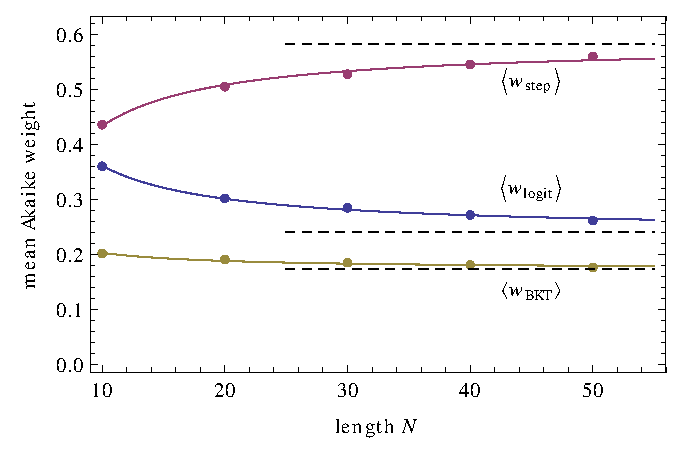
\includegraphics{mean-weights.eps}
  \caption{Mean Akaike weights for the three models, 
   $P_\mathrm{step}$, $P_\mathrm{logistic}$, and $P_\mathrm{BKT}$, 
   when fit to randomly generated data of length $n$.
   (Each mean is calculated by averaging over 10,000 random bit sequences.)
   Also shown is a fit to a function of the form $a+b/n$ and
   a dashed line marking the asymptotic value $a$.
   Note that the large differences between the weights persist
   in the $n\to\infty$ limit.}\label{meanweight}
\end{figure}

Since we know that AIC (or BIC) is only strictly valid in
the asymptotic limit $n\to\infty$, it is useful to see if
the large differences persist as $n$ is increased.
If we average over the 10,000 weights and plot the average weight 
as a function of $n$, we find
that the differences between the weights persist
in the $n\to\infty$ limit;  see Fig.~\ref{meanweight}.
If we fit the average weights to a constant plus $1/n$;
the fits are:
%
\begin{eqnarray}
 \langle w_\mathrm{step}\rangle &=& 0.58 - \frac{1.50}{n} \\
 \langle w_\mathrm{logistic}\rangle &=& 0.24 + \frac{1.2}{n} \\
 \langle w_\mathrm{BKT}\rangle &=& 0.17+\frac{0.30}{n} \; .
\end{eqnarray}
%
This shows that AIC, in the asymptotic limit $n\to\infty$, 
still favors  $P_\mathrm{step}$ over the other two models
when used to evaluate randomly generated data.

If we repeat this analysis with BIC, we would still
find that the weights converge to a constant value with 
$1/n$ leading errors.  The only difference is that the logistic
model has a larger weight than the other two. 
The differences between the weights of the three models still persist
in the $n\to\infty$ limit.

\subsection{Summary}

In conclusion, we obtain some surprising results when we compare
the three models,  $P_\mathrm{step}$, $P_\mathrm{logistic}$, and
$P_\mathrm{BKT}$, using individual student data.   We see that AIC
weakly favors the step model over the logistic model in a fashion 
that one might expect.  However, in an unexpected fashion, we see 
that both are strongly favored over the BKT model.
We see that this effect persists for
randomly generated data and is not due to an insufficient number
of opportunities (finite $n$ effect).

Moreover, for any bit sequence,  $P_\mathrm{BKT}$ {\em never}
fits the data better than $P_\mathrm{step}$.  Since 
both models have three parameters, this result holds for any maximum
likelihood-based criterion, including both AIC and BIC.  We don't have
an analytic proof for this result, 
but the numerical evidence (see Fig.~\ref{meanweight}) is quite strong.
In other words, even if one uses $P_\mathrm{BKT}$ (for some set of model parameters) 
to generate a bit sequence, one can
always adjust the parameters in $P_\mathrm{step}$ so that it
fits the bit sequence as well as, or better than, $P_\mathrm{BKT}$.


% How can we understand this?  Each model can be thought of as a
% set of functions.  One can ask how well each set of functions spans
% the space of all possible functions.  Evidently, the step model spans
% the space of all possible functions much better than the BKT model
% does.    Imagine that I choose some values for the parameters
% of the BKT model and then use the BKT model to construct a
% bit sequence $01011011\ldots$.  The 


What does this mean?  Let us think
more carefully about maximum likelihood.
If one uses a model to generate a single bit sequence, we cannot 
distinguish between that sequence and the exact probability function (the probability as a
function of $j$) that generated it.  At best, one can only
talk about probability functions that {\em may} have generated that sequence.
On the other hand, if one uses a particular probability function to generate a collection 
of infinitely many sequences, then we know the exact probability for each step.
Therefore, given the collection of sequences, one can uniquely determine the 
probability function that generated that collection. If that function comes from a
particular model $\mathcal{A}$ (for some choice of model parameters),
then we can safely conclude that model $\mathcal{A}$ is the correct model.

In other words, when we fit individual student data to a model (fitting
model parameters separately for each student), then we can make no
statements about what model is ``correct'' in the sense that it may
have generated the data.  We can only talk about a model being a good
fit in the sense that it is ``close'' to the data.
On the other hand, if we aggregate data from many students and fit to a
model (finding the best fit model parameters), then we can talk about
a model being correct in the usual sense  that it may have generated
the data.  

If we are interested in determining the effectiveness
of help given or of a particular student behavior,
we are more concerned about being ``close'' to
the student data than finding the correct theory of learning, so the
fact that the step model fits the data better than the logistic function and
the BKT model suggests that it may be useful for this purpose.
The idea is that any help given or student actions taken that
immediately precede step $L$ may have been more effective than
help given elsewhere, especially if the change in performance $1-s-g$
is large.

Finally, we see that the scatter plot of Akaike weights for student
data is remarkably similar to the scatter plots for the random model.
This suggests that the student data has a high degree of randomness,
and, in general, that study of the random model may be quite useful for better
understanding the student data.

%ACKNOWLEDGMENTS are optional
\section{Acknowledgments}

Funding for this research was provided by the Pittsburgh Science of
Learning Center which is funded by the National Science Foundation
award No. SBE-0836012. 

%
% The following two commands are all you need in the
% initial runs of your .tex file to
% produce the bibliography for the citations in your paper.
\bibliographystyle{abbrv}
\bibliography{education-modeling}
%Generated by bibtex from your ~.bib file.  Run latex,
%then bibtex, then latex twice (to resolve references)
%to create the ~.bbl file.  Insert that ~.bbl file into
%the .tex source file and comment out
%the command \texttt{{\char'134}thebibliography}.

\end{document}
